\section{Exercises on Minimum Spanning Trees Problems}

\paragraph{}
\begin{quote}
	GTC has been provided with 50 locations to connect in a certain country. These locations need
to be connected in such a way that any two of these locations are able to communicate
with each other. All the connections need not be direct. Due to high bandwidth
requirements, GTC will use high capacity cables for the connections, and wants to
know the costs of laying the cable under various circumstances. In Figure \ref{graph2-1} we
have schematically depicted the 50 locations and all possible direct connections. The
numbers attached to the connections in Figure \ref{graph2-1} refer to the distances (in 10 kilometer
units) between locations. The cost of the cable is \texteuro 5,000 per kilometer.
\end{quote}

\begin{figure}[H]
	\centering
	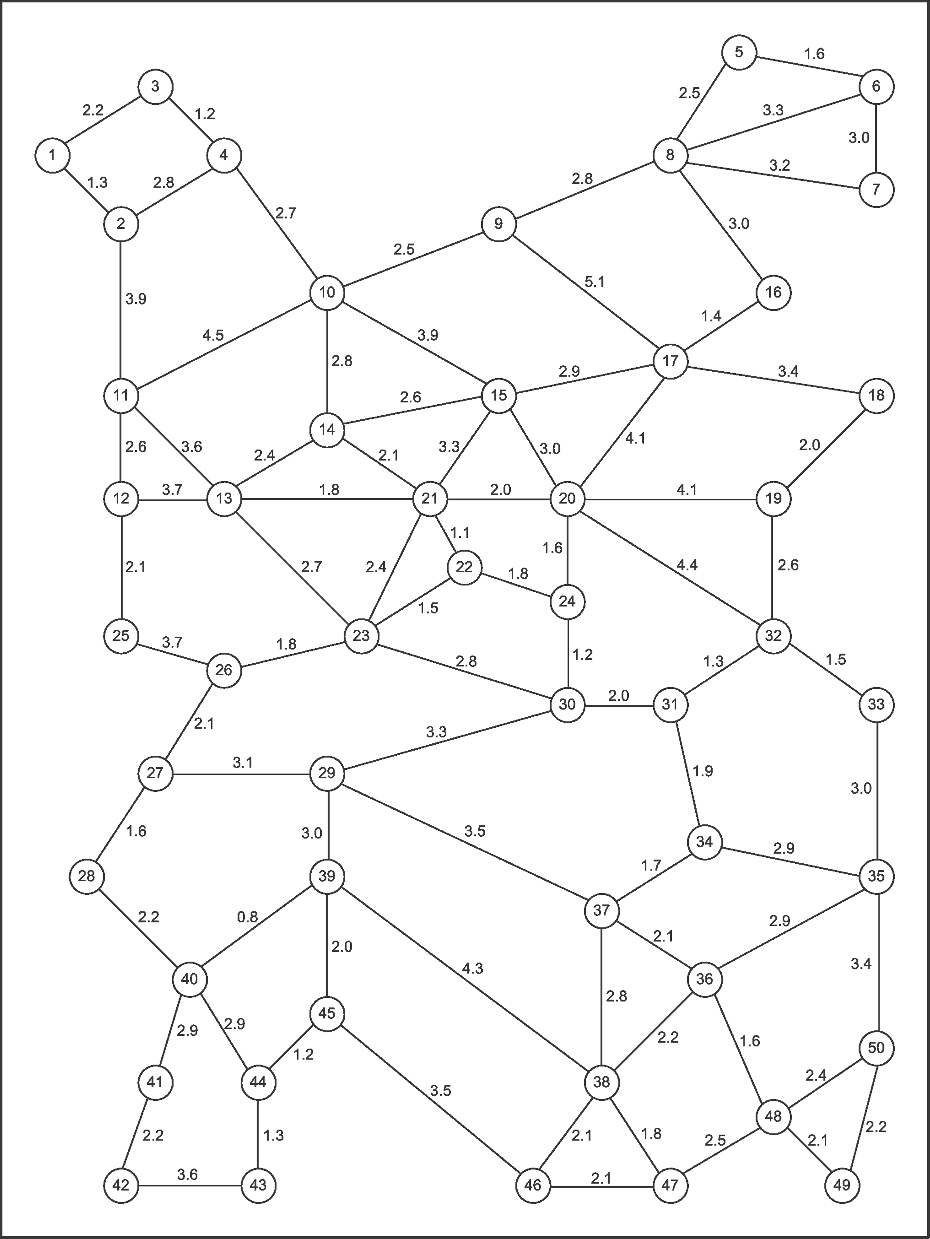
\includegraphics[scale=0.5]{./img/graph2-1.png}
	\caption{Schematic map with 50 locations (distances in 10 kilometer units, costs in \texteuro5,000per kilometer)}
	\label{graph2-1}
\end{figure}

\subsection{Problem 2.1. Reliable Cable Connections}
\begin{enumerate}[(a)]
\item \begin{quote}Calculate the minimum length of cable needed to connect all locations in Figure
\ref{graph2-1}. Also give the list of connections that are used for the cabling.\end{quote}

\paragraph{}
	Let's consider a graph with vertices corresponding to the locations in a country and edges corresponding to possible direct connections. This graph is undirected because the cable connections transmit data in both directions and weighted --- weight of a particular edge connecting two vertices is a length of a possible direct connection in km between two corresponding locations.

\paragraph{}
	Then the sought for system of connections between locations with a minimum length of cable required is a minimum spanning tree in a described graph. Indeed in the spanning tree there is a unique path between each pair of vertices so there are no redundant connections and every location is able to communicate with other locations using cables of this system. Also by definition the sum of weights of edges in a MST is minimal possible among all the spanning trees of the graph so this system requires the minimal possible length of cable to connect all the location thus the minimal possible sum of money because we pay equally \texteuro 5,000 for every km.

\paragraph{}
	MST problem can be solved efficiently using Kruskal's algorithm. The edges of the MST (the connections between locations in the country) are listed in figure \ref{mst1}. The length of cable needed to connect all locations is 1000 km which results in a \texteuro 5,000,000 total price of the system.

\begin{figure}[H]
	\centering
	\begin{multicols}{5}
(1,~2), (1,~3), (3,~4), (4,~10), (5,~6), (5,~8), (6,~7), (8,~9), (9,~10), (10,~14), (11,~12), (11,~13), (12,~25), (13,~21), (14,~15), (14,~21), (15,~17), (16,~17), (18,~19), (19,~32), (20,~24), (21,~22), (22,~23), (22,~24), (23,~26), (24,~30), (26,~27), (27,~28), (28,~40), (29,~39), (30,~31), (31,~32), (31,~34), (32,~33), (34,~35), (34,~37), (36,~37), (36,~38), (36,~48), (38,~46), (38,~47), (39,~40), (39,~45), (40,~41), (41,~42), (43,~44), (44,~45), (48,~49), (49,~50)
	\end{multicols}
	\caption{List of connections in a minimum cost communication system}
	\label{mst1}
\end{figure}

\item \begin{quote}GTC regrets that the locations 9 and 17 are not directly connected in the solution
of part (a). There can be taken two ways to get 9 and 17 connected --- adding
a direct cable between 9 and 17 to the solution of Problem 2.1(a) and deleting a
most expensive connection in the cycle thus created, or repeating the calculations
of Problem 2.1(a) with the extra restriction that the connection 9~--~17 has to be
in the new solution. Compare both methods. Will both methods always give the
same result? Explain your answer.\end{quote}

\paragraph{}
	Both methods will always give the same result. The 9~--~17 edge will produce a cycle 9~--~10~--~14~--~15~--~17~--~9 where the heaviest edge besides 9~--~17 is 15~--~17 that will be removed from the tree. The resulting tree will have a total cable length of 1022 km with a total cost of \texteuro 5,110,000.

\paragraph{}
	The equivalence of both methods can be easily shown if one follows the steps of the Kruskal's algorithm. According to the Kruskal's algorithm the MST is built incrementally edge by edge in the ascending order of weights. The important part is that on each iteration of the algorithm the current edge is either added to the MST or disregarded since it produces a cycle. So if an edge was once added to MST than it wouldn't be deleted later. Thus we can consider the iterative consecutive process of building cycle 9~--~10~--~14~--~15~--~17~--~9 edge by edge instead of adding 9~--~17 to the complete MST. Since the algorithm iterates through edges in the ascending order of weights the last two edges to consider will be 15~--~17 and 9~--~17 as the heaviest ones. But one can make these two edges equally suitable for the Kruskal algorithm by increasing the weight of 15~--~17 to match the weight of 9~--~17. After that the algorithm can naturally pick the edge 9~--~17 thus building a new spanning tree with total weight increased by exactly the weight difference of edges 9~--~17 and 15~--~17. But increasing the weight of 15~--~17 is the exact equivalence of adding 9~--~17 to spanning tree as the first edge from this cycle since the Kruskal's algorithm will add the remaining edges in ascending order of weight thus leaving the 15~--~17 behind as the second heaviest.

\item \begin{quote}The cable system designed in part (a) is not very reliable, in the sense that there
is only one connection between any pair of locations. Why is this so?
Determine, by inspection, a most vulnerable connection in your solution to part
(a), in the sense that if the cable on this connection breaks down, the most number
of pairs of locations will not be able communicate anymore.\end{quote}

\paragraph{}
	The cable system designed in part (a) is not very reliable because the cable connections form a tree. As a result there is a unique path between every pair of vertices. Thus the removal of any edge will cause the graph to lose connectivity.

\paragraph{}
	The ``vulnerability'' of the direct connection in the described sense can be calculated in a single traverse of a tree using DFS. Starting the DFS naturally roots the tree thus it's becomes easy to calculate the answer for the edge by computing the size of the subtree of the deeper vertex of the edge. The size of the other subtree (to the other part of the edge) is computed as a difference between the total number of vertices and the size of the first subtree. The sought for ``vulnerability'' is a product of sizes of these subtrees.

\paragraph{}
	The most vulnerable connection is 21~--~22. The break down of this connection will cause 589 pairs of locations (31 on the one side of the edge and 19 on another) to lose contact with each other.

\item \begin{quote}Design a reliable cable connection, in the sense that if the cable between any
two locations breaks down, there is still a connection (although possibly indirect)
between these locations. Is your design the cheapest possible?\end{quote}

\paragraph{}
	The cable system will be reliable in a described sense if it's corresponding graph has no bridges~--- is 2-edge-connected. It is known that the problem of finding minimum spanning subgraphs with these property is NP-hard \cite{garey79}. Since it's hard to find the optimal solution~--- minimum spanning 2-edge-connected subgraph, we will compute the minimal spanning 2-edge-connected subgraph (a removal of any edge in such subgraph leads to lose of 2-edge-connectivity). For this task the simple $O(m(n+m))$ ($n$~--- number of vertices, $m$~--- number of edges) algorithm is suitable~--- we try to delete each edge from the graph and if after the removal the 2-edge-connectivity is preserved than we delete this edge permanently. Else we add this edge to the resulting spanning subgraph. The edges of this subgraph are listed in figure \ref{reliable1}. The cable length of the system equals 1373 km with a total cost of \texteuro 6,865,000.

\begin{figure}[H]
	\centering
	\begin{multicols}{5}
(1,~2), (1,~3), (2,~11), (3,~4), (4,~10), (5,~6), (5,~8), (6,~7), (7,~8), (8,~9), (8,~16), (9,~10), (11,~12), (11,~13), (12,~25), (13,~14), (14,~15), (15,~17), (16,~17), (17,~18), (18,~19), (19,~20), (19,~32), (20,~21), (21,~23), (22,~23), (22,~24), (23,~26), (24,~30), (25,~26), (27,~28), (27,~29), (28,~40), (29,~30), (29,~37), (30,~31), (31,~32), (32,~33), (33,~35), (34,~35), (34,~37), (35,~36), (35,~50), (36,~38), (38,~39), (39,~40), (40,~41), (41,~42), (42,~43), (43,~44), (44,~45), (45,~46), (46,~47), (47,~48), (48,~49), (49,~50)
	\end{multicols}
	\caption{List of connections in a reliable communication system}
	\label{reliable1}
\end{figure}


\end{enumerate}